\documentclass[a4paper, titlepage, 10pt]{article}
\usepackage[T2A]{fontenc}
\usepackage[utf8]{inputenc}
\usepackage[english, russian]{babel}
\usepackage{indentfirst}
\usepackage{amsmath}
\usepackage{graphicx}
\usepackage{float}
\hoffset=-2.1cm
\voffset=-1.6cm
\setlength{\parindent}{1cm}
\textwidth= 16cm
\textheight = 24cm
\newcommand{\HRule}{\rule{\linewidth}{0.5mm}}
\begin{document}
\begin{titlepage}
\begin{center}
% Upper part of the page
\textsc{\LARGE ГУАП}\\[2cm]
\textsc{\LARGE Кафедра антенн и эксплуатации радиоэлектронной 
 аппаратуры}
\\[1cm]


 \begin{flushleft} \large
  \emph{Отчёт} \\
   \emph{защищен с оценкой}
   \\[0.5cm]
   \emph{Преподаватель}\\[-4mm]
   \HRule
\end{flushleft}
\begin{flushright}
Должность, уч. степень, звание \ \ \ \ \ \ \ подпись, дата \ \ \ \ \ \ \ инициалы, фамилия \\[10mm]
\end{flushright}

\textsc{\Large Отчёт о лабораторной работе №5:} \\[1cm]
\textsc{\Large ИССЛЕДОВАНИЕ ПОВЕРХНОСТЫХ ВОЛН, РАСПРОСТРАНЯЮЩИХСЯ ВДОЛЬ ПЛОСКИХ ЗАМЕДЛЯЮЩИХ СИСТЕМ.}\\[1.5cm]
% Title

% Author and supervisor

\begin{flushleft} \large
\emph{Работу выполнил:}\\
Студент\\ гр. 5025.\\[-4mm]
\HRule
\end{flushleft}
\begin{flushright}
подпись, дата \ \ \ \ \ \ \ инициалы, фамилия \\[10mm]
\end{flushright}

\vfill
% Bottom of the page
Санкт-Петербург, {\today}
\end{center}
\end{titlepage}
\appendix
\section*{Цели лабораторной работы.}
\indent Целью данной лабораторной работы является изучение поверхностных волн, способов возбуждения некоторых поверхностых волн, конструкций и принцыпов действия некоторых типов линий передачи поверхностных волн. Экспериментальное определение коэффициента замедления и поперечного коэффициента затухания поверхностной волны, распространяющейся вдоль диэлектрической пластины, расположенной на металлической подложке, коэффициента замедления и поперечного коэффициента затухания поверхностной волны, распространяющейся вдоль металлической гребенчатой (гофрированной) структуры.
\appendix
\section*{Схема лабораторной работки.}
Ниже представлена функциональная схема лабораторной установки для проведения данной лабораторной работы:
\\
\begin{center}
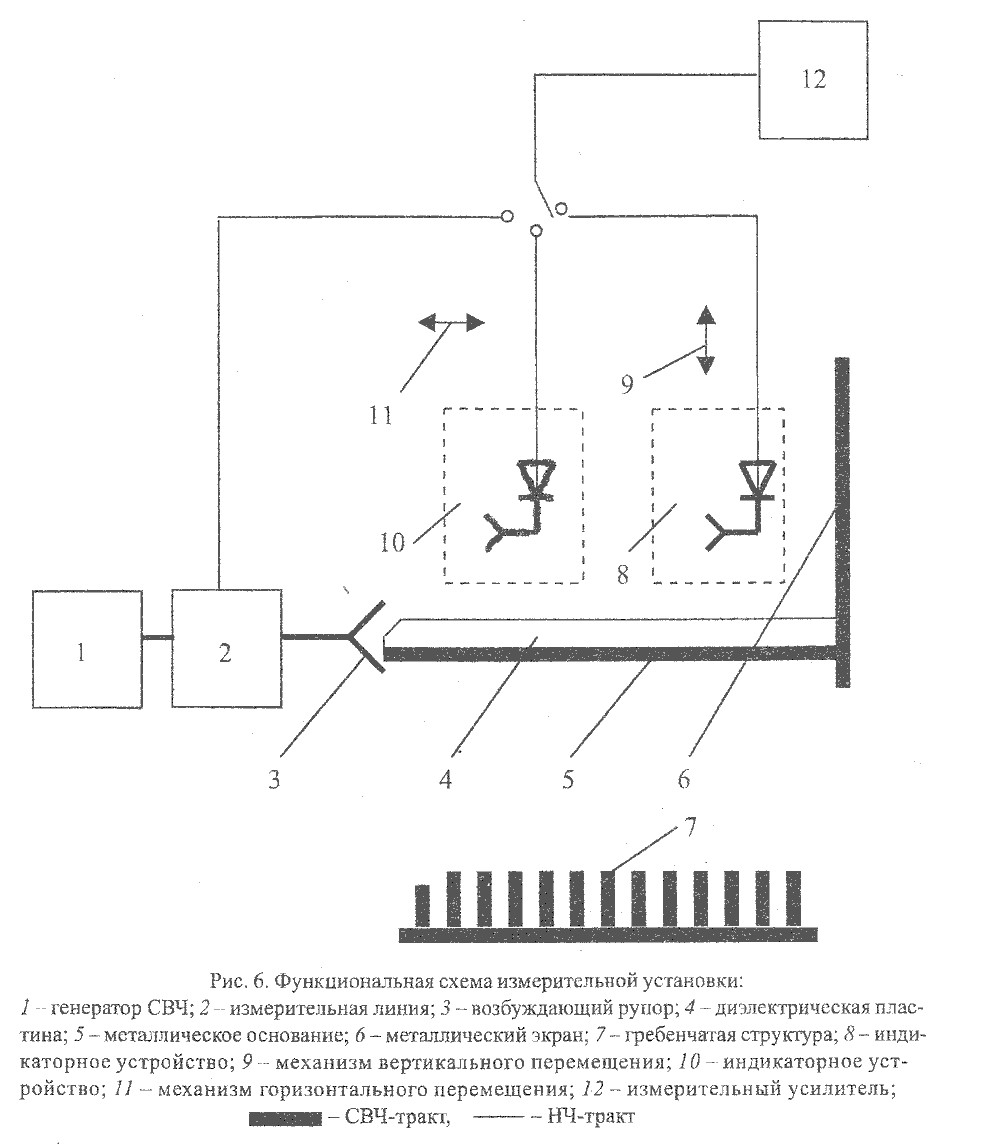
\includegraphics[width=0.5\textwidth]{07.jpeg}
\end{center}
Поверхностные волны возбуждаются рупором 3, для согласования возбуждающего устройства устройства входящие в в полость рупора части ЛП (линии передачи) выполнены в виде клина длиной (2-3). \\Индикаторное устройство 8, предназначенное для измерения поперечного (в направлении нормали к поверхности ЛП) распределения напряжённости электрического поля, предсталяет из себя отрезок прямоугольного волновода, нагруженный на детекторную секцию, открытый конец волновода играет роль антенны. Индикаторное устройство 10, предназначенное для измерения продолного распределения напряжённости электрического поля, представляет из себя ассиметричный вибратор, нагруженный на детекторную секцию. Так же следует отметить, что оба детектора измеряют только вертикальную составляющую вектора электрической напряжённости. Измеритель 12 можно по очереди подключать к обеим индикаторным секциям 8 и 10 или к низкочастотному выходу волновой измерительной линии 2. 
\\[2cm]
\vfill


\appendix
\section*{Результаты измерений в таблицах.}

\begin{table}[h!]
 \begin{center}
  \begin{tabular}{|l|l|l|}
  \hline
   1ый минимум(см)  &  2ой минимум(см)  &  3ий минимум(см)  \\
  \hline
   \( Z_{1.1} = 0.5 \) , \( Z_{1.2} = 1.1 \) & \( Z_{1.2} = 2.8 \) , \( Z_{1.2} = 3.5 \) & \( Z_{1.3} = 5.1 \) , \( Z_{1.3} = 5.8 \) \\
  \hline
  \( Z_{min1} = 0.75 \) & \( Z_{min2} = 3.25 \) & \(Z_{min3} = 5.5 \) \\
  \hline

  \end{tabular}
  \caption{Вычисление методом ,,вилки'' , для нахождения длины волны.}
 \end{center}
\end{table}

Ниже представлена формула для вычисления длины волны и вычисленное значение:
\begin{center}
\( \Lambda_{B} = \frac{2 \cdot (Z_{min2} - Z_{min1}) + 2 \cdot (Z_{min3} -Z_{min2}) }{ 2} = 2,375\) см \\[1cm]
\end{center}

\begin{minipage}{0.4\textwidth}
\begin{center}
 \begin{tabular}{|l|l|l|}
  \hline
  Z,мм & \( \gamma \) & \( \sqrt{\gamma \over  \gamma_{max}} \) \\
  \hline
  200 & \( 10 \cdot 2^3 \) & \( 0.623 \) \\
  \hline
  203 & \( 25 \cdot 2^3 \) & \( 1.000 \) \\
  \hline
  206 & \( 12 \cdot 2^3 \) & \( 0.693 \) \\
  \hline
  209 & \( 12 \) & \( 0.245 \) \\
  \hline
  212 & \( 0 \) & \( 0.000 \) \\
  \hline
  215 & \( 28 \cdot 2^2 \) & \( 0.748 \) \\
  \hline
  218 & \( 20 \cdot 2^3 \) & \( 0.894 \) \\
  \hline
  221 & \( 10 \cdot 2^3 \) & \( 0.632 \) \\
  \hline
  224 & \( 20 \) & \( 0.387 \) \\
  \hline
  227 & \( 0 \) & \( 0 \) \\
  \hline
  230 & \( 17 \cdot 2^2 \) & \( 0.583 \) \\
  \hline
  233 & \( 12 \cdot 2^3 \) & \( 0.692 \) \\
  \hline
  236 & \( 36 \cdot 2^2 \) & \( 0.848 \) \\
  \hline
  239 & \( 14 \cdot 2^1 \) & \( 0.374 \) \\
  \hline
  242 & \( 0 \) & \( 0 \) \\
  \hline
  245 & \( 10 \cdot 2^2 \) & \( 0.447 \) \\
  \hline
  248 & \( 44 \cdot 2^2 \) & \( 0.938 \) \\
  \hline
  251 & \( 34 \cdot 2^2 \) & \( 0.825 \) \\
  \hline
  254 & \( 16 \cdot 2^1 \) & \( 0.4 \) \\
  \hline
  257 & \( 0 \) & \( 0 \) \\
  \hline
  260 & \( 25 \cdot 2^1 \) & \( 0.5 \) \\
  \hline
 \end{tabular}
\\[1cm]
 \begin{tabular}{|l|l|l|}
  \hline
  X,мм & \( \gamma \) & \( \sqrt{\gamma \over  \gamma_{max}} \) \\
  \hline
  310 & \( 14 \cdot 2^5 \) & \( 1.000 \) \\
  \hline
  312 & \( 12 \cdot 2^5 \) & \( 0.926 \) \\
  \hline
  314 & \( 25 \cdot 2^4 \) & \( 0.945 \) \\
  \hline
  316 & \( 10 \cdot 2^4 \) & \( 0.598 \) \\
  \hline
  318 & \( 23 \cdot 2^3 \) & \( 0.641 \) \\
  \hline
  320 & \( 13 \cdot 2^3 \) & \( 0.482 \) \\
  \hline
  322 & \( 34 \cdot 2^2 \) & \( 0.551 \) \\
  \hline
  324 & \( 20 \cdot 2^2 \) & \( 0.423 \) \\
  \hline
  326 & \( 38 \cdot 2 \) & \( 0.412 \) \\
  \hline
  328 & \( 10 \cdot 2 \) & \( 0.211 \) \\
  \hline
  330 & \( 4 \) & \( 0.094 \) \\
  \hline
 \end{tabular}
 
\end{center}
\end{minipage}
\hfill
\begin{minipage}{0.4\textwidth}
\begin{center}
 \begin{tabular}{|l|l|l|}
  \hline
  Z,мм & \( \gamma \) & \( \sqrt{\gamma \over  \gamma_{max}} \) \\
  \hline
  200 & \( 34 \) & \( 0.595 \) \\
  \hline
  203 & \( 22 \cdot 2^1 \) & \( 0.677 \) \\
  \hline
  206 & \( 15 \cdot 2^2 \) & \( 0.791 \) \\
  \hline
  209 & \( 48 \cdot 2^1 \) & \( 1.000 \) \\
  \hline
  212 & \( 42 \) & \( 0.661 \) \\
  \hline
  215 & \( 10 \) & \( 0.323 \) \\
  \hline
  218 & \( 8 \cdot 2^1 \) & \( 0.408 \) \\
  \hline
  221 & \( 18 \cdot 2^1 \) & \( 0.612 \) \\
  \hline
  224 & \( 24 \cdot 2^1 \) & \( 0.707 \) \\
  \hline
  227 & \( 28 \) & \( 0.540 \) \\
  \hline
  230 & \( 10 \) & \( 0.323 \) \\
  \hline
  233 & \( 14 \cdot 2^1 \) & \( 0.540 \) \\
  \hline
  236 & \( 34 \cdot 2^1 \) & \( 0.842 \) \\
  \hline
  239 & \( 32 \cdot 2^1 \) & \( 0.816 \) \\
  \hline
  242 & \( 12 \cdot 2^1 \) & \( 0.5 \) \\
  \hline
  245 & \( 26 \) & \( 0.520 \) \\
  \hline
  248 & \( 38 \) & \( 0.630 \) \\
  \hline
  251 & \( 14 \cdot 2^1 \) & \( 0.540 \) \\
  \hline
  254 & \( 10 \cdot 2^1 \) & \( 0.456 \) \\
  \hline
  257 & \( 14 \) & \( 0.382 \) \\
  \hline
  260 & \( 0 \) & \( 0 \) \\
  \hline
 \end{tabular}
\\[1cm]
 \begin{tabular}{|l|l|l|}
  \hline
  X,мм & \( \gamma \) & \( \sqrt{\gamma \over  \gamma_{max}} \) \\
  \hline
  310 & \( 40 \cdot 2^4 \) & \( 1.000 \) \\
  \hline
  312 & \( 30 \cdot 2^4 \) & \( 0.866 \) \\
  \hline
  314 & \( 20 \cdot 2^4 \) & \( 0.707 \) \\
  \hline
  316 & \( 8 \cdot 2^4 \) & \( 0.447 \) \\
  \hline
  318 & \( 14 \cdot 2^3 \) & \( 0.418 \) \\
  \hline
  320 & \( 20 \cdot 2^2 \) & \( 0.354 \) \\
  \hline
  322 & \( 20 \cdot 2^1 \) & \( 0.25 \) \\
  \hline
  324 & \( 14 \) & \( 0.148 \) \\
  \hline
  326 & \( 0 \) & \( 0 \) \\
  \hline
 \end{tabular}
\end{center}
\end{minipage}

\appendix
\section*{\\[1cm]Расчёт \( \xi\) и \(  \alpha \).}
\( \lambda_{0} = \frac{\Lambda_B}{\sqrt{1 + \frac{\Lambda_B}{\lambda_{kp}}} } = 1.928\)


\appendix
\section*{Графики экспериментальной зависимости \( \gamma \).}

\begin{figure}[h!]
 \centering
 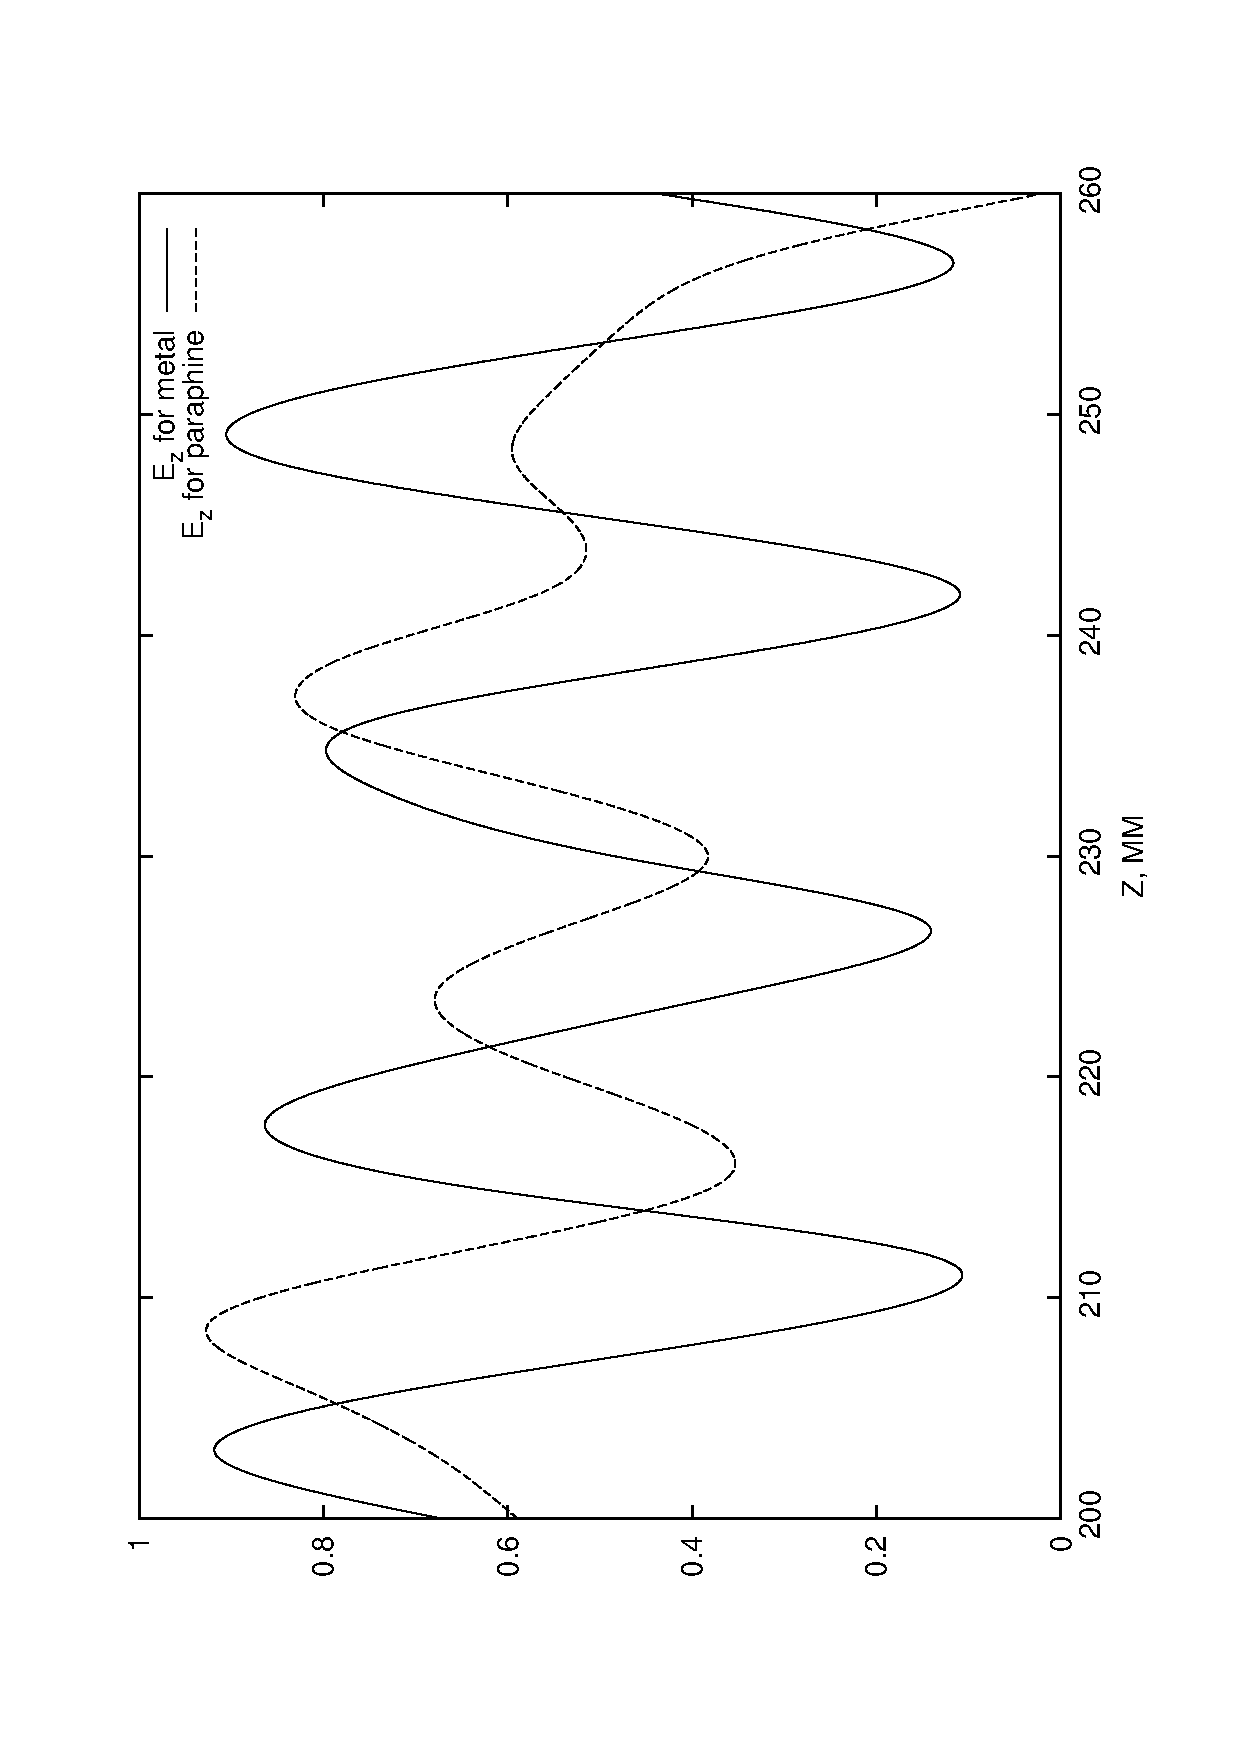
\includegraphics[angle = 270,width=0.7\textwidth]{Ez}
 \caption{Графики зависимости \( \gamma \) в продольном сечении от расстояния Z.}
\end{figure}

\begin{figure}[h!]
 \centering
 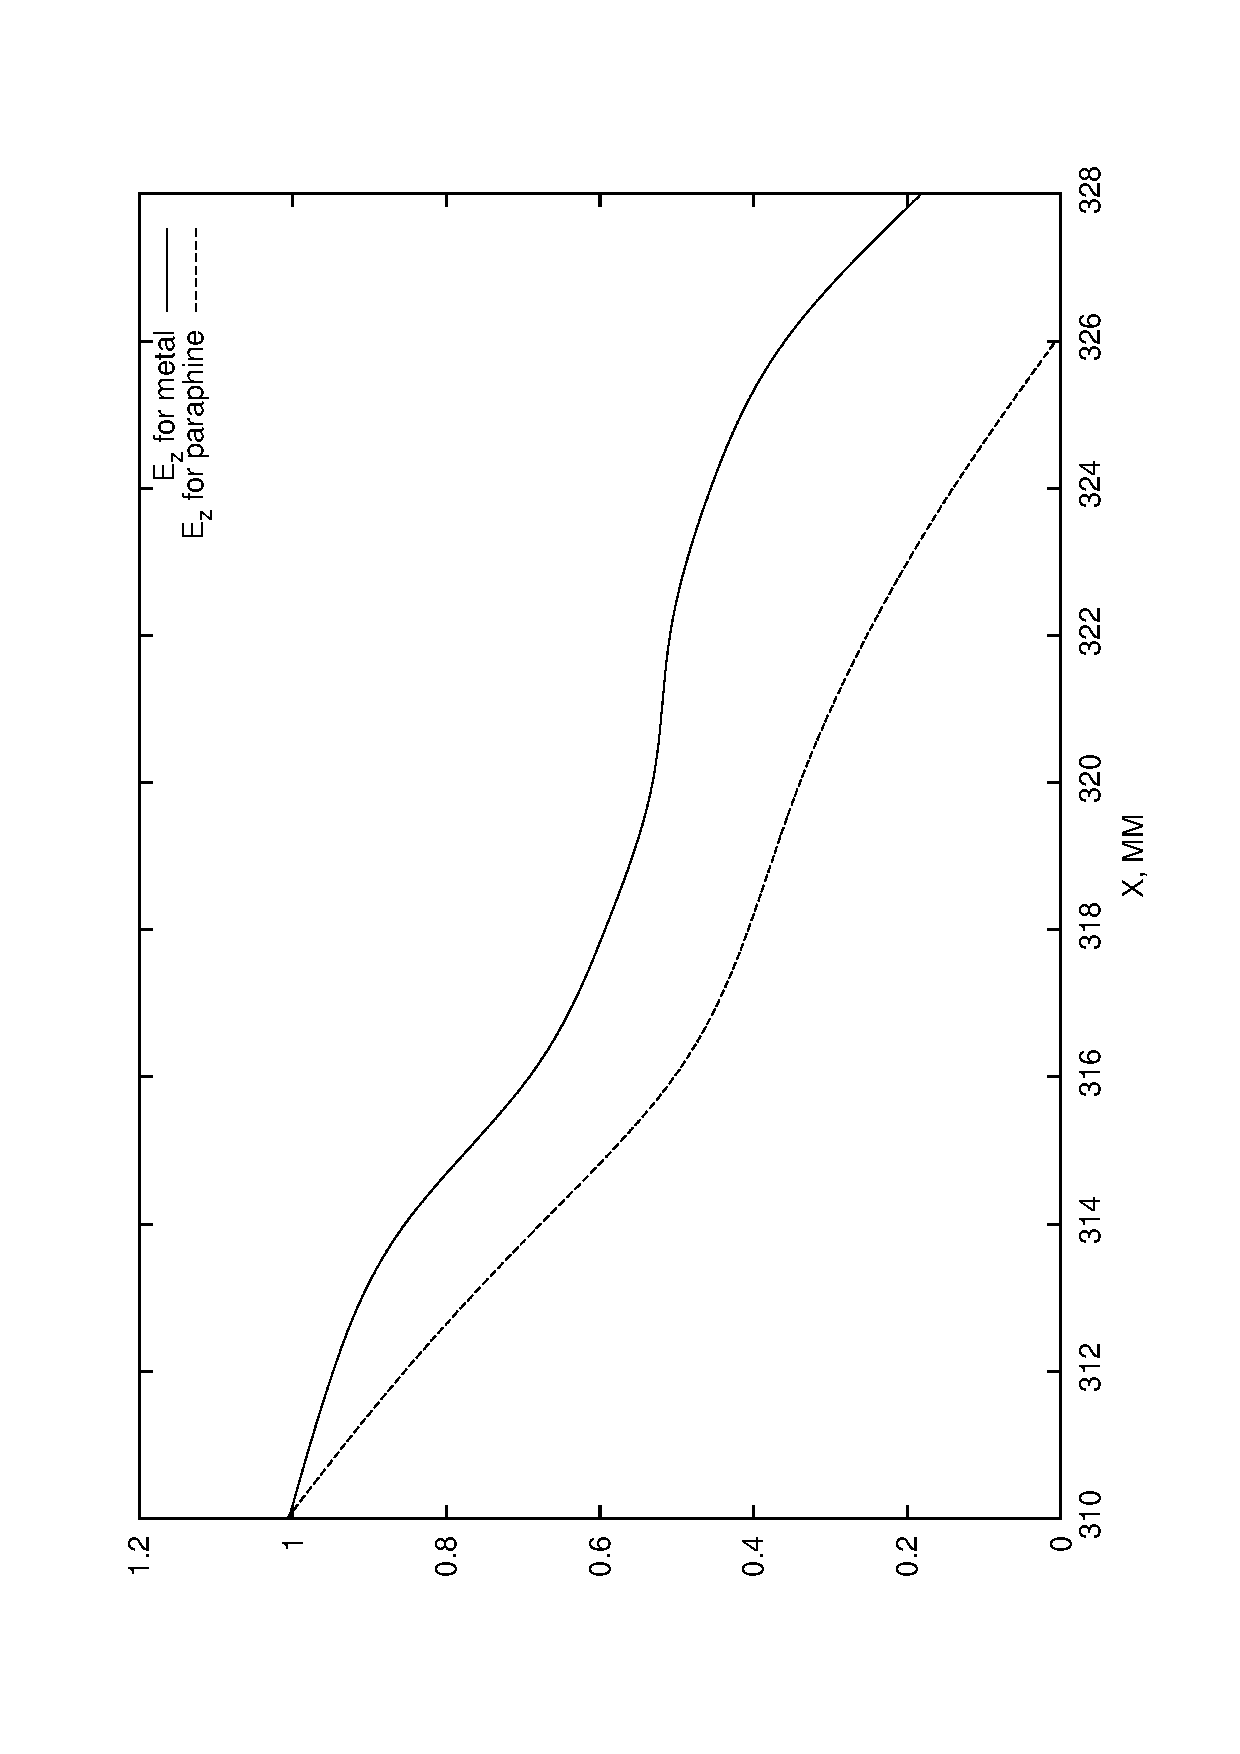
\includegraphics[angle = 270,width=0.7\textwidth]{Ex}
 \caption{Графики зависимости \( \gamma \) в продольном сечении от расстояния X.}
\end{figure}

\appendix
\section*{Выводы по проделанной работе.}
В результате выполнения данной лабораторной работы удалось вычислить значени длины волны на линии передачи, вычислить коэффициент затухания для продольного и поперечного сечений. Так же удалось построить графики практической зависимости напряжённости Е от расстояния Z и X.
\end{document}